\documentclass[conference]{IEEEtran}
\usepackage{amsmath,amssymb}
\usepackage{graphicx}
\usepackage{booktabs}
\usepackage{cite}
\usepackage{url}
\usepackage[hidelinks]{hyperref}

\begin{document}

\title{Why Adaptive Combinations of Tail-Risk Forecasts Fail:\\
Pre-Registered Evidence of Level Drift in Indian Equities}

% Author names and affiliations to be agreed by the authors before submission.
\author{\IEEEauthorblockN{Author One}
\IEEEauthorblockA{Affiliation\\ email}
\and
\IEEEauthorblockN{Author Two}
\IEEEauthorblockA{Affiliation\\ email}}

\maketitle

\begin{abstract}
Learned, state-dependent combinations of Value-at-Risk (VaR) and Expected Shortfall (ES) forecasts promise to adapt to market conditions, yet in practice they often fail to beat simple averages. We study why. We compare a range-based heterogeneous autoregressive (HAR) model, equal-weight and Taylor (2020) combinations of six econometric risk models, and neural gates trained on the strictly consistent FZ0 joint VaR--ES loss, on Indian equities. After development on 20 assets, we pre-registered four hypotheses and tested them once on 27 National Stock Exchange stocks that were never used before, over 2023--2026. A gate without level control is significantly worse than HAR (Diebold--Mariano $-3.47$, Holm-adjusted $p=0.001$), and the same gate with a penalty that keeps its learned scale near one is significantly better than the uncontrolled gate ($-3.19$, $p=0.002$; better for 25 of 27 stocks). The uncontrolled gate's loss grows with the level shift it learns (correlation $-0.45$ across 108 stock-years) and its ES is rejected by the Acerbi--Sz\'ekely test for 9 of 27 stocks. HAR does not beat simple combinations, and a power analysis shows more stocks would not change that. The results extend forecast-combination and location-shift theory to learned tail-risk combinations: level drift, not a lack of state information, is the main cause of failure.
\end{abstract}

\begin{IEEEkeywords}
Value-at-Risk, expected shortfall, forecast combination, FZ loss, HAR, pre-registration, Indian equities
\end{IEEEkeywords}

\section{Introduction}

Banks and asset managers forecast daily VaR and ES, and the Basel framework now places ES at 97.5\% at the centre of market-risk capital. Since ES became jointly elicitable with VaR \cite{fissler2016}, models can be trained and compared on a strictly consistent joint loss, the FZ0 loss of Patton, Ziegel and Chen \cite{patton2019}. This has made combinations of VaR/ES forecasts an active topic: Taylor \cite{taylor2020} and Storti and Wang \cite{storti2023} estimate combination weights by minimising joint scores, and Taylor and Wang \cite{taylorwang2025} combine large pools of methods.

A natural next step is to let the weights depend on the market state, for example through a small neural network that maps volatility, implied volatility and recent model losses to weights, as feature-based model averaging does for point forecasts \cite{montero2020}. The forecast-combination literature gives reasons to be cautious: estimated weights add bias and variance that can exceed their gains \cite{claeskens2016,smith2009,elliott2026}, and simple averages are hard to beat \cite{stock2004}. Location shifts are a main source of forecast failure \cite{clements1998}. Whether these mechanisms explain the behaviour of learned tail-risk combinations has not, to our knowledge, been tested.

This paper makes three contributions.
\begin{itemize}
\item \textbf{A pre-registered evaluation.} We fixed hypotheses, decision rules, the asset list and the code commit, and published them before downloading the test data. To our knowledge this is the first pre-registered study of VaR/ES forecast combination. Pre-registration separates confirmatory from exploratory evidence \cite{nosek2018} and is rare in volatility forecasting.
\item \textbf{A tested failure mechanism.} Learned gates fail mainly through \emph{level drift}: they learn a multiplicative level shift from the training years that does not carry forward. Controlling the level removes most of the failure. We confirm this out of sample and measure the mechanism directly.
\item \textbf{Evidence for Indian equities.} On 27 never-used NSE stocks, a range-based HAR model, equal weights, Taylor combinations and a level-controlled gate are statistically indistinguishable; the uncontrolled gate and the single GARCH-family models are excluded from the Model Confidence Set.
\end{itemize}

All data, code and the pre-registration are public.\footnote{Repository: \url{https://github.com/amateurcoder015/har-anchored-tail-risk}; earlier development study: \url{https://github.com/amateurcoder015/state-dependent-gate-trained-on-FZ-loss}.}

\section{Related Work}

\textit{Volatility and tail-risk models.} GARCH-family models \cite{bollerslev1986,nelson1991,glosten1993} and RiskMetrics EWMA \cite{riskmetrics1996} remain standard; Hansen and Lunde \cite{hansen2005} found few models beat GARCH(1,1) for point volatility. HAR models \cite{corsi2009} and range-based variance estimators \cite{parkinson1980,garman1980,rogers1991} are strong for daily risk, and Meng and Taylor \cite{meng2020} use intraday range data for VaR and ES. Quantile approaches such as CAViaR \cite{engle2004} and the joint models of \cite{patton2019} fit VaR and ES directly.

\textit{Combining VaR and ES forecasts.} Taylor \cite{taylor2020} proposes minimum-score and relative-score combining for VaR and ES; Storti and Wang \cite{storti2023} add weighted quantiles; Taylor and Wang \cite{taylorwang2025} study large pools. Weights in these methods are fixed or depend on past performance only.

\textit{Why combinations fail.} The forecast combination puzzle has been explained by estimation error in the weights \cite{smith2009,claeskens2016} and by small potential gains relative to that error \cite{elliott2026}. Location shifts, which change the mean of the forecast target, are a leading cause of forecast failure \cite{clements1998}. We test whether the same mechanism appears in learned, state-dependent tail-risk combinations.

\section{Methods}

\subsection{Data}
Daily open, high, low, close and adjusted close prices from Yahoo Finance, 2015-01-01 to 2026-09-30, and the India VIX. Returns are log changes of the adjusted close. Raw files are frozen with SHA-256 hashes. No-trade rows and Diwali \emph{Muhurat} sessions (about one hour of trading on an exchange holiday) are removed. Every daily return above 10\% in absolute value is reviewed; a row is dropped only for an unadjusted split, bonus or demerger. The \emph{development universe} has 20 assets (NIFTY 50, NIFTY Bank and 18 stocks). The \emph{fresh universe} has 27 stocks, three per sector, none used before (Section~\ref{sec:prereg}).

\subsection{Base models and combinations}
Six base models produce a VaR/ES pair each day: EWMA with filtered historical simulation \cite{riskmetrics1996}; GARCH, EGARCH and GJR-GARCH with Student-$t$ errors \cite{bollerslev1986,nelson1991,glosten1993}; HAR on log Garman--Klass variance \cite{corsi2009,garman1980} with empirical tails; and a model scaling the India VIX. All are refitted every 21 trading days on an expanding window and forecast out of sample from 2020. HAR is our anchor model R0. Baselines are the equal-weight mean, the median, previous-best selection, and Taylor's minimum-score and relative-score combinations \cite{taylor2020}.

\subsection{Learned gates}
A gate maps a state vector $x_t$ (trailing model losses, realized and implied volatility, volatility of volatility, the variance risk premium, expiry-calendar features and lagged returns, all measured before $t$) to convex weights $w^Q_t, w^S_t$ over the six models and a scale $g_t=\exp(0.5\tanh(\cdot))$:
\begin{align}
\mathrm{VaR}_t &= g_t \textstyle\sum_i w^Q_{i,t}\,\mathrm{VaR}_{i,t},\\
\mathrm{ES}_t &= g_t\big(\textstyle\sum_i w^Q_{i,t}\,\mathrm{VaR}_{i,t} + \sum_i w^S_{i,t}(\mathrm{ES}_{i,t}-\mathrm{VaR}_{i,t})\big),
\end{align}
which extends Taylor's minimum-score form \cite{taylor2020} to state-dependent weights and guarantees $\mathrm{ES}_t\le\mathrm{VaR}_t<0$. It is a one-hidden-layer network trained on mean FZ0 loss \cite{patton2019} with yearly walk-forward folds (train from 2020, validate on the next year, test on the year after), early stopping and five seeds. The \emph{level-controlled} gate adds a penalty $\lambda_g\,\overline{(\log g_t)^2}$ with $\lambda_g=10$ fixed in advance.

\subsection{Anchor-based alternatives}
R1 fits $\mathrm{VaR}_t=-\exp(a+b^\top z_t)$, $\mathrm{ES}_t=\mathrm{VaR}_t(1+e^{c})$ on log daily, weekly and monthly Garman--Klass, Parkinson and Rogers--Satchell variances and India VIX by minimising FZ0. R2 applies a bounded correction to HAR: $\mathrm{VaR}_t=\mathrm{VaR}^{\mathrm{HAR}}_t e^{c_v}$ and $\mathrm{ES}_t=\mathrm{VaR}_t+(\mathrm{ES}^{\mathrm{HAR}}_t-\mathrm{VaR}^{\mathrm{HAR}}_t)e^{c_s}$, with $c=0.25\tanh(f(x_t))$ from a small network or a linear map, trained on FZ0 with penalties on the size and on the average of the corrections.

\subsection{Evaluation}
The test period is 2023-01-01 to 2026-09-30 and the main tail level is $\alpha=2.5\%$. Forecasts are compared on the cross-stock average FZ0 loss per date with Diebold--Mariano tests \cite{diebold1995} using Newey--West variance and the correction of Harvey, Leybourne and Newbold \cite{harvey1997}, and with the Model Confidence Set \cite{hansen2011}. VaR is backtested with the Kupiec \cite{kupiec1995}, Christoffersen \cite{christoffersen1998} and dynamic quantile \cite{engle2004} tests, and ES with the Acerbi--Sz\'ekely $Z_2$ test \cite{acerbi2014}, with critical values simulated for each stock's sample length.

\section{Development and Pre-Registration}\label{sec:prereg}

All design choices were made on the development universe and logged. There, HAR had the lowest pooled FZ0 loss at $\alpha=1\%$ and 2.5\% and was within 0.002 of the lowest at 5\% (Table~\ref{tab:fz0}); a first version of R2 learned an average VaR shrink of about 6\% and lost to HAR, and penalising the average correction brought it level with HAR. R1 was worse than HAR at every level.

We then fixed four hypotheses, each a one-sided DM test at $\alpha=2.5\%$ with Holm correction \cite{holm1979} at family-wise level 0.05: H1, HAR beats equal weights; H2, HAR beats Taylor minimum-score combining; H3, HAR beats the gate without level control; H4, the level-controlled gate beats the uncontrolled gate. The hypotheses, the 27-stock list, the outlier rule and the code commit were tagged and pushed to the public repository before any fresh data was downloaded, and the study was run once. One deviation is disclosed: an earlier public draft of the design named R1 and R2 as the main hypotheses; they were replaced after development and before the fresh download, and we report them below. The fresh stocks were chosen by sector and size rather than by the mechanical list rule in the draft. The outlier rule removed one row (the Vedanta demerger ex-date, 2026-04-30).

\section{Results}

\begin{table}[t]
\centering
\caption{Pooled mean FZ0 loss (lower is better), test period 2023-01 to 2026-09}
\label{tab:fz0}
\footnotesize
\setlength{\tabcolsep}{3pt}
\begin{tabular}{lrrrrrr}
\toprule
& \multicolumn{3}{c}{Development (20)} & \multicolumn{3}{c}{Fresh (27)}\\
\cmidrule(lr){2-4}\cmidrule(lr){5-7}
Method & 1\% & 2.5\% & 5\% & 1\% & 2.5\% & 5\%\\
\midrule
R2-MLP & -2.9716 & -3.2572 & -3.4799 & -2.9107 & -3.1844 & -3.3970 \\
R2-linear & -2.9662 & -3.2542 & -3.4795 & -2.9090 & -3.1824 & -3.3967 \\
HAR (R0) & -2.9765 & -3.2589 & -3.4787 & -2.9166 & -3.1808 & -3.3948 \\
Taylor min.\ score & -2.9631 & -3.2495 & -3.4796 & -2.9065 & -3.1799 & -3.3954 \\
Taylor rel.\ score & -2.9584 & -3.2450 & -3.4752 & -2.9027 & -3.1787 & -3.3939 \\
Equal weights & -2.9568 & -3.2404 & -3.4675 & -2.9106 & -3.1752 & -3.3881 \\
Gate (level control) & -2.9629 & -3.2543 & -3.4763 & -2.9037 & -3.1743 & -3.3920 \\
HAR-X FZ (R1) & -2.9137 & -3.2369 & -3.4680 & -2.8380 & -3.1479 & -3.3772 \\
Gate (no level control) & -- & -- & -- & -- & -3.1460 & -- \\

\bottomrule
\end{tabular}
\end{table}

\begin{table}[t]
\centering
\caption{Pre-registered hypotheses, fresh universe, $\alpha=2.5\%$}
\label{tab:hyp}
\footnotesize
\setlength{\tabcolsep}{3pt}
\begin{tabular}{llrrrl}
\toprule
& Hypothesis (lower loss first) & DM & $p$ & Holm $p$ & Supported\\
\midrule
H1 & HAR $<$ equal weights & -0.53 & 0.300 & 0.600 & No \\
H2 & HAR $<$ Taylor min.\ score & -0.09 & 0.463 & 0.600 & No \\
H3 & HAR $<$ gate (no level control) & -3.47 & $<$0.001 & 0.001 & Yes \\
H4 & Gate (level control) $<$ gate (no level control) & -3.19 & $<$0.001 & 0.002 & Yes \\

\bottomrule
\end{tabular}
\end{table}

\subsection{Confirmatory results}
Table~\ref{tab:hyp} reports the registered tests. H3 and H4 are supported: the uncontrolled gate is significantly worse than HAR and than the same gate with level control. H1 and H2 are not supported: HAR, equal weights and Taylor's combinations are statistically indistinguishable. At the 10\% level the Model Confidence Set contains HAR, equal weights, both Taylor combinations, previous-best selection and the level-controlled gate, and excludes the single GARCH-family models, EWMA, the VIX model, the median and the uncontrolled gate.

The originally planned hypotheses are not supported on the fresh data either: R1 is significantly worse than HAR (DM $3.57$), and neither R2 variant beats HAR (one-sided $p=0.21$ and $0.35$), although R2 with a neural correction has the lowest point estimate at 2.5\% and 5\% and beats HAR for 17 of 27 stocks.

\subsection{Robustness and mechanism}
The following analyses were not pre-registered. H3 holds at $\alpha=1\%$, 2.5\% and 5\%, and H4 at 2.5\% and 5\% ($p=0.057$ at 1\%). By year, H3 is significant in 2023, 2024 and 2026 with the same sign in 2025; H4 is significant in 2024 and 2026, has the same sign in 2025 and the opposite, non-significant sign in 2023 (Table~\ref{tab:rob}, Fig.~\ref{fig:year}). The level-controlled gate beats the uncontrolled gate for 25 of 27 stocks.

Fig.~\ref{fig:mech} shows the mechanism. Across 108 stock-years, the more the uncontrolled gate shrinks its scale, the larger its loss relative to HAR (correlation $-0.45$; $-0.45$ within years and $-0.51$ within stocks; descriptive, as stock-years are not independent). On average it shrinks VaR by about 6\%, a level learned from the training years. Shrunken forecasts understate tail losses: its ES is rejected by the $Z_2$ test for 9 of 27 stocks, against 3 for the level-controlled gate, and its VaR exceptions cluster, with the dynamic quantile test rejecting for 11 stocks against 2 (Table~\ref{tab:bt}).

A power projection from the observed effect sizes and cross-stock correlation shows the achievable DM statistic for H1, H2 and R2 versus HAR is capped below 1.1 in absolute value however many stocks are added, because the loss differences are correlated across stocks. A larger sample would therefore not separate these methods.

\begin{table}[t]
\centering
\caption{H3 and H4 by tail level and by test year (one-sided $p$, not corrected)}
\label{tab:rob}
\footnotesize
\begin{tabular}{lrrrr}
\toprule
& \multicolumn{2}{c}{H3} & \multicolumn{2}{c}{H4}\\
\cmidrule(lr){2-3}\cmidrule(lr){4-5}
& DM & $p$ & DM & $p$\\
\midrule
0.01 & -2.32 & 0.010 & -1.58 & 0.057 \\
0.025 & -3.47 & $<$0.001 & -3.19 & $<$0.001 \\
0.05 & -2.55 & 0.005 & -2.66 & 0.004 \\
\midrule
2023 & -3.24 & $<$0.001 & 0.49 & 0.687 \\
2024 & -1.77 & 0.039 & -1.91 & 0.029 \\
2025 & -0.96 & 0.169 & -1.00 & 0.158 \\
2026 & -2.25 & 0.013 & -3.23 & $<$0.001 \\

\bottomrule
\end{tabular}
\end{table}

\begin{table}[t]
\centering
\caption{Backtests, fresh universe, $\alpha=2.5\%$ (number of the 27 stocks rejected at 5\%)}
\label{tab:bt}
\footnotesize
\setlength{\tabcolsep}{4pt}
\begin{tabular}{lrrrr}
\toprule
Method & Hit rate & Kupiec & DQ & $Z_2$\\
\midrule
HAR (R0) & 0.026 & 5 & 3 & 5 \\
Equal weights & 0.022 & 4 & 3 & 0 \\
Taylor min.\ score & 0.026 & 5 & 6 & 4 \\
Gate (level control) & 0.025 & 2 & 2 & 3 \\
Gate (no level control) & 0.029 & 3 & 11 & 9 \\
HAR-X FZ (R1) & -- & -- & -- & 10 \\
R2-MLP & -- & -- & -- & 4 \\

\bottomrule
\end{tabular}
\end{table}

\begin{figure}[t]
\centering
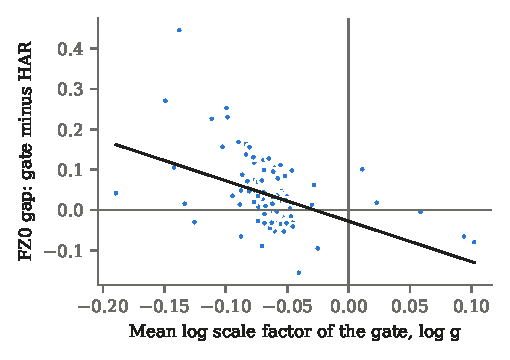
\includegraphics[width=\columnwidth]{figures/mechanism.pdf}
\caption{Uncontrolled gate, one point per stock-year: mean log scale factor against the gate's mean FZ0 loss minus HAR's. Line: least-squares fit.}
\label{fig:mech}
\end{figure}

\begin{figure}[t]
\centering
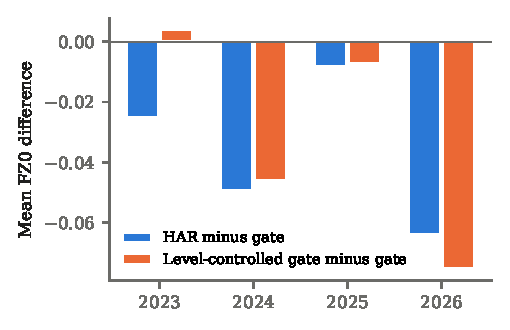
\includegraphics[width=\columnwidth]{figures/by_year.pdf}
\caption{Mean FZ0 differences by test year, pooled over 27 stocks. Negative values favour the first-named method.}
\label{fig:year}
\end{figure}

\section{Discussion}

The evidence points to one mechanism. A learned gate can adjust both the mix of models and the overall level of risk. The mix is useful but small; the level is where it overfits, because in the training years after the COVID shock the base models tended to over-forecast risk, and the gate learned to shrink them. When conditions changed, the learned shrinkage persisted. This is the tail-risk version of the location-shift failures described by Clements and Hendry \cite{clements1998} and of the estimation-error explanations of the combination puzzle \cite{claeskens2016,elliott2026}. A penalty that keeps the learned level near one removes most of the damage, and a bounded correction of a strong anchor (R2) does no harm, but neither beats a simple combination significantly.

For practitioners the implication is direct: a learned combination of VaR/ES forecasts should not be allowed to rescale risk freely. Level control, or an anchor that is refitted regularly, is a minimum requirement.

\textit{Limitations.} The data are daily Yahoo Finance prices for one market; intraday realized measures may change the ranking. The test period is under four years, and India-specific events (the 2024 election, the Vedanta demerger) affect some years. The robustness and mechanism analyses are exploratory. The pre-registration is a public repository tag rather than a registry entry.

\section{Conclusion}

In a pre-registered test on 27 Indian stocks never used in development, learned state-dependent combinations of VaR and ES forecasts failed through level drift, and controlling the learned level fixed most of the failure. Simple combinations, a range-based HAR model and a level-controlled gate were statistically tied, and a power analysis showed more data would not separate them. We release the data, code, development log and pre-registration so others can test the same mechanism in other markets.

\bibliographystyle{IEEEtran}
\bibliography{refs}

\end{document}
